
%%%%%%%%%%%%%%%%%%%%%%% file typeinst.tex %%%%%%%%%%%%%%%%%%%%%%%%%
%
% This is the LaTeX source for the instructions to authors using
% the LaTeX document class 'llncs.cls' for contributions to
% the Lecture Notes in Computer Sciences series.
% http://www.springer.com/lncs       Springer Heidelberg 2006/05/04
%
% It may be used as a template for your own input - copy it
% to a new file with a new name and use it as the basis
% for your article.
%
% NB: the document class 'llncs' has its own and detailed documentation, see
% ftp://ftp.springer.de/data/pubftp/pub/tex/latex/llncs/latex2e/llncsdoc.pdf
%
%%%%%%%%%%%%%%%%%%%%%%%%%%%%%%%%%%%%%%%%%%%%%%%%%%%%%%%%%%%%%%%%%%%


\documentclass[runningheads,a4paper]{llncs}

\usepackage{amssymb}
\setcounter{tocdepth}{3}
\usepackage{graphicx}
\usepackage{rotating}

\usepackage{url}
\urldef{\mailsa}\path|kruza@ufal.mff.cuni.cz|    
\newcommand{\keywords}[1]{\par\addvspace\baselineskip
\noindent\keywordname\enspace\ignorespaces#1}

\begin{document}

\mainmatter  % start of an individual contribution

% first the title is needed
\title{Czech parliament meeting recordings as ASR training data}

% a short form should be given in case it is too long for the running head
\titlerunning{Czech parliament meeting recordings as ASR training data}

% the name(s) of the author(s) follow(s) next
%
% NB: Chinese authors should write their first names(s) in front of
% their surnames. This ensures that the names appear correctly in
% the running heads and the author index.
%
\author{Jan Oldřich Krůza}
%
\authorrunning{Jan Oldřich Krůza}
% (feature abused for this document to repeat the title also on left hand pages)

% the affiliations are given next; don't give your e-mail address
% unless you accept that it will be published
\institute{Institute of Formal and Applied Linguistics,\\
Faculty of Mathematics and Physics,\\
Charles University
\mailsa\\
\url{ufal.mff.cuni.cz}}

%
% NB: a more complex sample for affiliations and the mapping to the
% corresponding authors can be found in the file "llncs.dem"
% (search for the string "\mainmatter" where a contribution starts).
% "llncs.dem" accompanies the document class "llncs.cls".
%

\toctitle{Czech parliament meeting recordings as ASR training data}
\tocauthor{Jan Oldřich Krůza}
\maketitle


\begin{abstract}
I present a way to leverage the stenographed recordings of the Czech parliament
meetings for purposes of training a speech-to-text system. The article presents
a method for scraping the data, acquiring word-level alignment and selecting
reliable parts of the imprecise transcript. Finally, I present an ASR system
trained on these data.
\keywords{speech corpus, speech recognition, czech}
\end{abstract}


\section{Introduction}

Training data for speech recognition is always a demanded commodity, especially
if it is free. There are for sure already some free Czech corpora fit for speech
recognition training:
\begin{itemize}
\item{
    Vystadial\cite{vystadialarticle} with its 77 hours of VoIP
    calls\cite{vystadialdata}, 
}
\item{
    The Prague Database of Spoken Czech\cite{pdtscarticle} with its 122 hours
    of richly annotated spontaneous dialogues\cite{pdtscdata},
}
\item{
    The Czech Senior COMPANION Expressive Speech Corpus with its 5 hours
    of professionally spoken utterances by a single speaker\cite{companiondata},
}
\item{
    Otázky Václava Moravce: 35 hours of transcribed recordings of the
    Czech TV talk show\cite{ovmdata},
}
\item{
    STAZKA, a set of speech recording from vehicles with its 35 hours of
    background noise and utterances\cite{stazkadata},
}
\item{
    Spoken Corpus of Karel Makoň\cite{kruuza2012making} with its 70 hours of
    manually transcribed spontaneous speech by a single speaker\cite{makondata},
}
\item{and possibly others that I am not aware of.}
\end{itemize}

The Czech parliament meeting recordings represent a publicly available dataset
of high-quality audio recordings of contemporary Czech in consistent low-noise
audio quality worth almost 4000 hours of downloadable material, about 2800 hours
with the overlaps subtracted. Extracting
training data for speech recognition systems would provide a corpus at least
one order greater in length than those so far publicly available.

Verily, I am not the first person to attempt using these recordings for speech
recognition. The Department of Cybernetics of University of West Bohemia
developed an automatic online subtitling system for the meetings in
2006\cite{pspsubs} and as a result, an 88-hour subset annotated by high-quality
automatic transcript has been released for speech recognition training
purposes\cite{pspdata}.

I attempt to use the official stenographic transcripts available for all the
talks so that it can be a new entry in the above list, on par in quality and
excelling in size.

\section{Data Preparation}

Since the source data is publicly available and in the public domain, I merely
provide the scripts for downloading and building the corpus. The algorithms and
parameters used are described in this section.

\subsection{Scraping}

Regrettably, the data are to my best knowledge only available in human-readable
form. The transcript is not clearly distinguished in the markup and is
interlaced with metainformation. My method of isolating the transcript is quite
crude but it covers the vast majority of cases. The criterion is to extract the
subtree of all nodes with HTML attribute \texttt{[align=justify]}, except HTML
elements \texttt{<b>}, which contain speaker identification.

The known shortcomings of this method are that 1) it discards the speaker
annotations, although it is valuable metainformation and 2) it skips some short
passages, e.g. references to other meetings, as can be seen in the meeting
from Feb. 12th 2020 10:10 -
10:20\footnote{https://www.psp.cz/eknih/2017ps/stenprot/040schuz/s040372.htm}.

\subsection{Alignment}

One of the obstacles in using the stenographic transcripts for training an ASR
system is the very loose alignment available. The recordings are all 14 minutes
long and have a 4-minute overlap. The corresponding transcript is thus aligned
in 10-minute blocks with a roughly 2-minute padding on each side of the audio.
Figure~\ref{fig:overlap} schematically shows the alignment of the stenographic
transcript to the audio and the overlap of the recordings.

\begin{figure}[htpb]
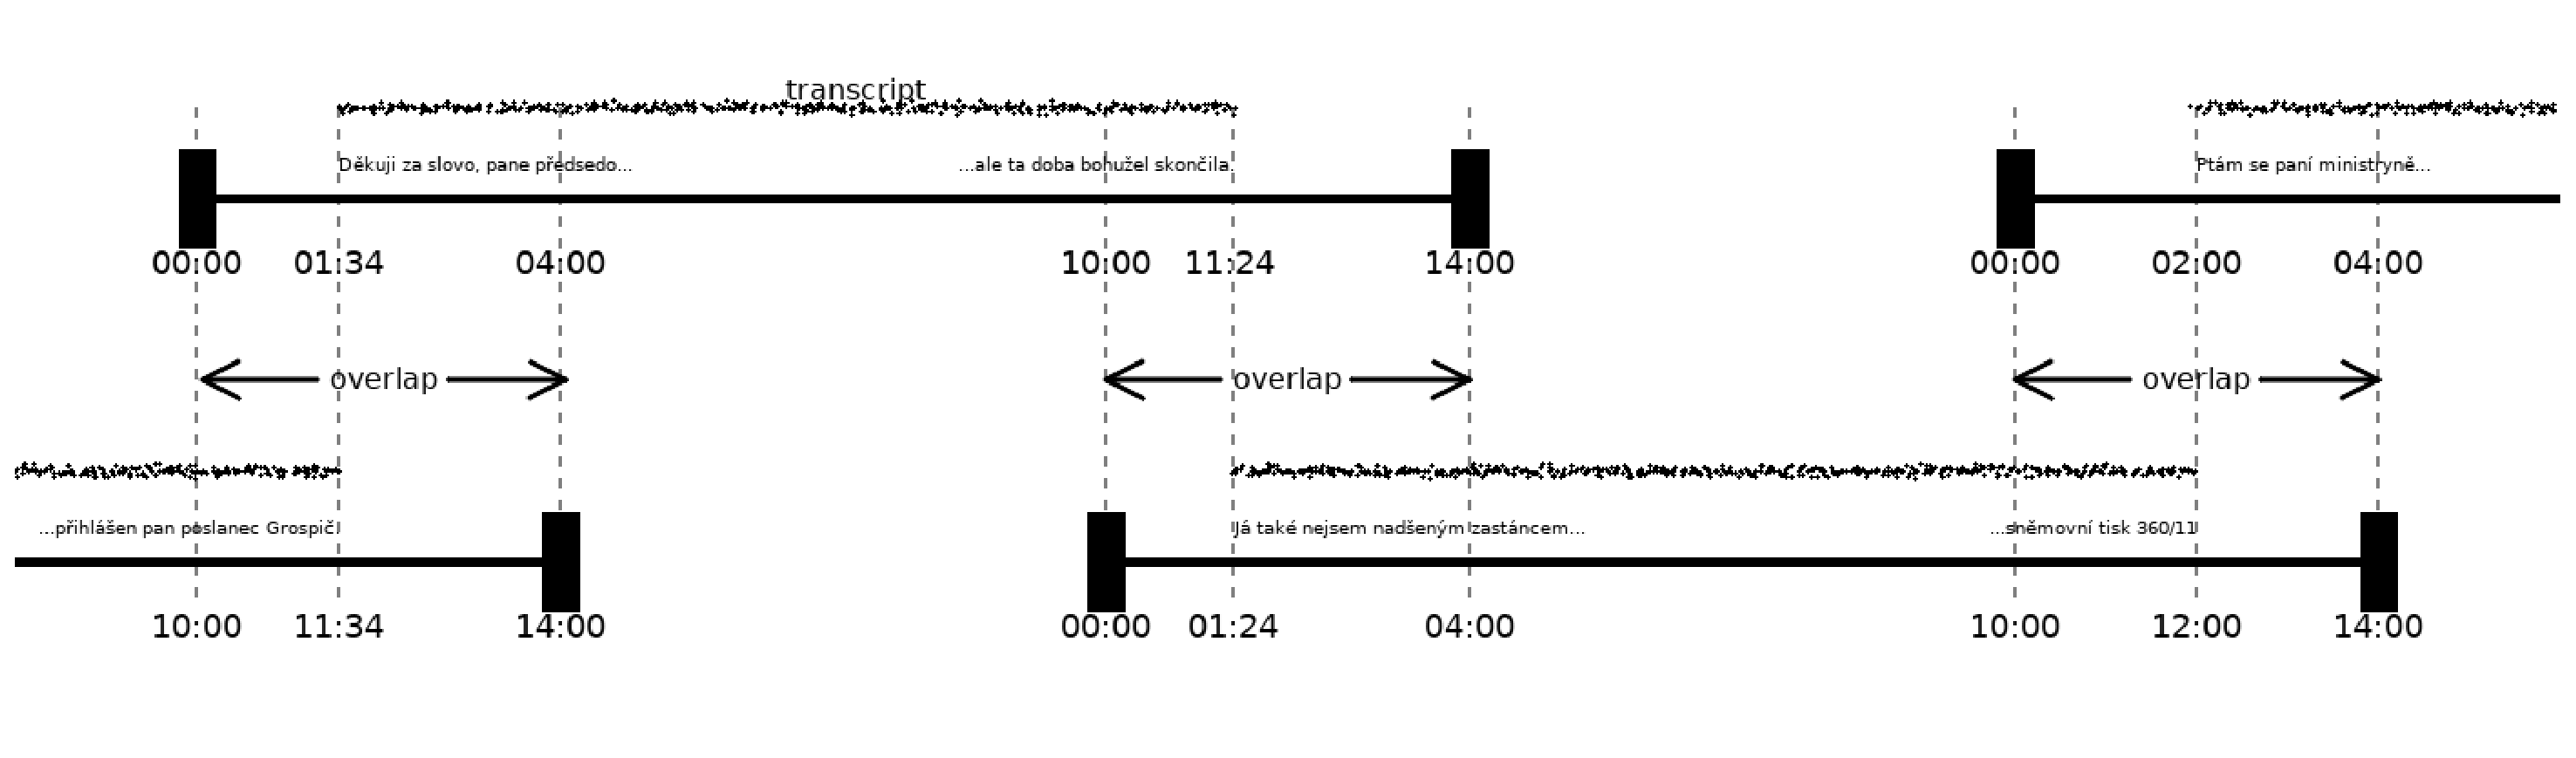
\includegraphics[scale=0.25]{rc/overlap.eps}
\caption{Alignment and overlap of audio files and transcript. The examples are
from Feb. 12th 2020 around 10 o'clock. The transcript corresponding to the
recording in the upper left covers audio positions 01:34 - 11:24. The one in the
lower right from 01:24 to 12:00.}
\label{fig:overlap}
\end{figure}

Systems for aligning long audio segments to their transcripts already exist,
like that of Moreno et al. 1998\cite{moreno1998recursive} or Hazen
2006\cite{hazen2006automatic}. They are both based on an already existing
automatically acquired transcript. I use this technique as well, though much
simplified.

I have used the dataset mentioned above\cite{pspdata} to train a GMM-based ASR
system, using the stenographs as training data for a language model. Using these
models, a word-level-aligned transcript of the whole set of recordings has been
acquired.

The predicted transcript and the stenographic one have then been compared for
Levenshtein distance, determining the edit operations needed to transform one
into the other. For each predicted word, an un-reliability score is then
computed as the number of edit operations taken on it divided by its length.
A reliability score is actually used, as 1 - un-reliability.
Figure~\ref{fig:align} shows how the stenographic transcript is aligned with the
audio on word level.

\begin{figure}[htpb]
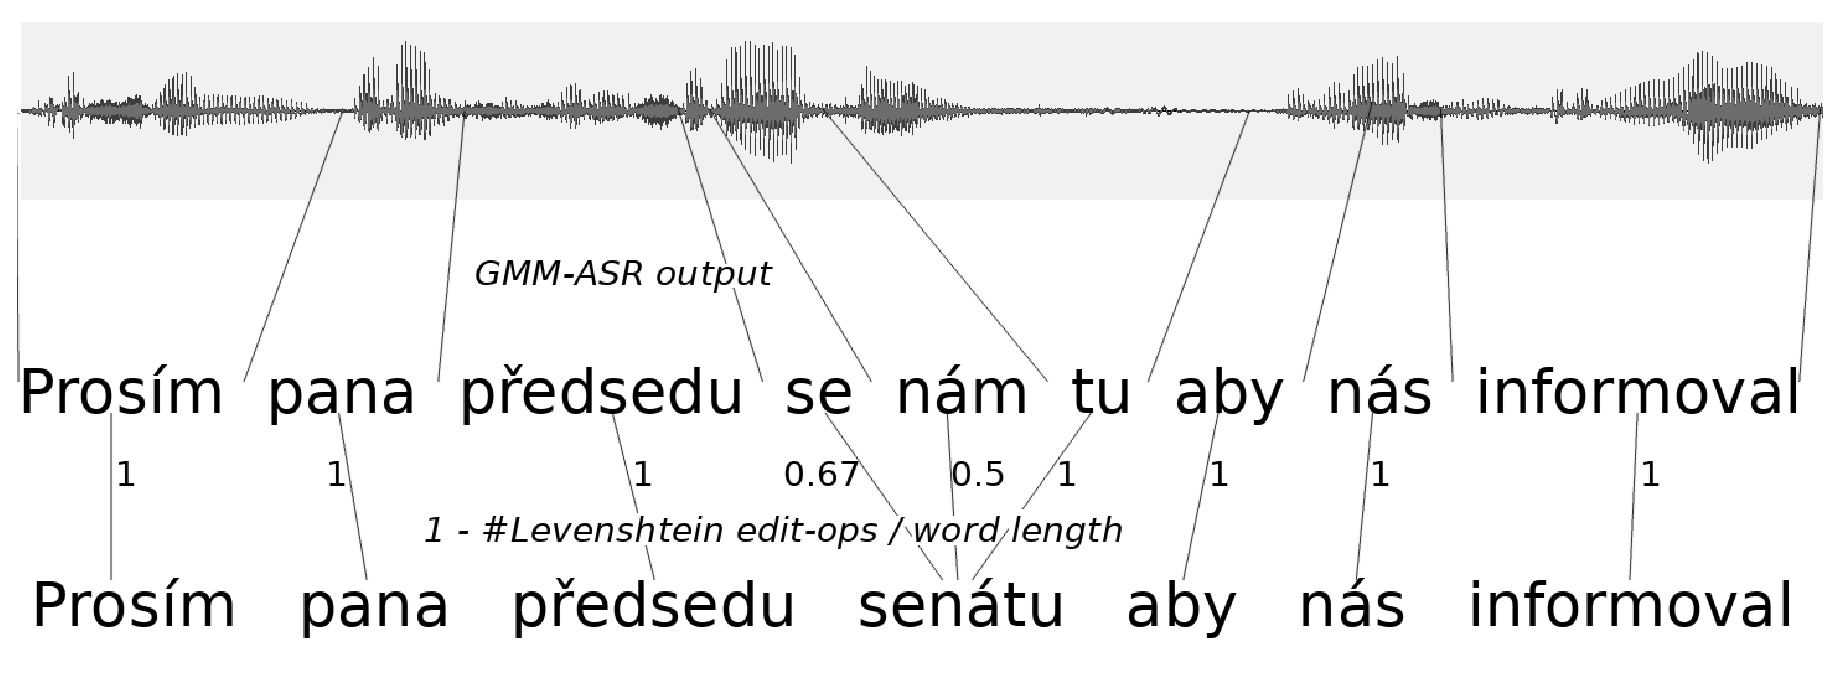
\includegraphics[scale=0.4]{rc/align.eps}
\caption{Schema of aligning the audio to the stenographic transcript on word
level.}
\label{fig:align}
\end{figure}

\subsection{Audio Segmentation}

To create a usable dataset for training a speech-to-text system, it is not
necessary to perfectly align the whole transcript. It is fine to just select the
reliable segments.

The criteria for good training samples are:
\begin{enumerate}
\item{100\% precise transcript,}
\item{roughly sentence-level length,}
\item{consistent length.}
\end{enumerate}

To ensure precise transcript, it is good to have the samples padded by some
silence, since the alignment may be a bit imprecise. The need to split at longer
pauses goes against the need to split at consistent, none-too-great lengths.

The problem of selecting the optimal set of silences so that the longest ones
are kept and split the recording in chunks of set length boundaries looks like
one for dynamic programming but I use a simpler approach: Start with a set of
all silences predicted by the forced alignment. Iterate over the silences
shortest-first and remove it if it doesn't break the constraints.

I have experimentally set the length boundaries to 12 - 30 seconds. The maximum
length could be decreased at the cost of more frequent splits in the middle of a
word.

\subsection{Training Samples Selection}

With the audio segmented and corresponding manual transcripts extracted, the
last step remaining is selecting which segments to include in the traning data.
Indeed, since the recordings have a 2-minute padding on each side for 10 middle
minutes, we must discard at the very least 40\% of the segments. I use the
following criteria for including a segment in the data:

\begin{enumerate}
\item{The first and last token have reliability at least 70\%,}
\item{The mean reliability of all tokens is at least 70\%,}
\item{The number of words is no less than five.}
\end{enumerate}

Minimum reliability of border tokens is considered to minimize the danger of
false alignment. Mean reliability is considered because it is OK for some
words to have reliability zero: there are enough errors in the prediction,
that's why we use the manual transcript after all. But if too many tokens have
too low reliability, then it is a sign of a suspicious segment. The number of
words has a minimum because with only a few words, the probability of
misalignment with good score is much greater than when there are enough words.

Why use mean reliability and not median? The way the reliability is computed,
considers the number of edit operations on one line in the automatic transcript.
In the case where there are many insertions, the reliability of one line can go
arbitrarily deep sub zero. So it can happen that there are several lines
extra words in the (mis)aligned chunk. The mean taps these.

\subsection{Data Extraction Summary}

All the constants and criteria are to be considered a baseline solution. They
all could be tweaked much more rigorously and solved much more soundly. However,
this simple solution readily yields a high-quality training dataset of 1058
hours. Of the total 539,057 segments, 142,530 (26\%) have been accepted to the
training dataset. Of the total 396,527 discarded segments, 350,258 (88\%) were
discarded because of the criterion of unreliable start or end.

Reducing the minimum reliability of the boundary words from 70\% to 50\% increases
the number of accepted chunks by 17\%. It adds 5\% segments
of the total number to the dataset. But if we consider that 40\% of the total
number of segments must be discarded because of audio padding, the gain is
acually 9\%. It is an option to increase the training data volume at the cost
of matching precision.

\section{ASR Based on the Dataset}

I have trained a standard DeepSpeech\cite{hannun2014deep} model with training :
dev : test ratio of 48 : 1 : 1; batch size 50; learning rate 0.0001. The
training took TODO epochs and the final WER on testing data from the corpus
itself was TODO.

\section{Conclusion}

I have presented a new corpus of spoken Czech suitable for training speech
recognition systems based on data in the public domain. The corpus size exceed
by an order the size of other freely available such corpora.

\section*{Acknowledgments}

This work has been using language resources developed, stored and distributed by
the LINDAT/CLARIAH project of the Ministry of Education, Youth and Sports of the
Czech Republic (project LM2018101).

\bibliographystyle{splncs}

\bibliography{citace}

\end{document}
